\documentclass[../../memoria.tex]{subfiles}

\begin{document}

\paragraph{}
Como se ha mencionado anteriormente, el despliegue de la solución se ha implementado a través de un script escrito en Bash (launch\_tfg.sh). En este apartado serán descritos los resultados de los pasos que sigue el script.

\begin{enumerate}
    \item El script está configuracio para lanzar el comando \textit{terraform apply -auto-approve}, lo que significa que no es necesearia una intervención manual que apruebe la aplicación de las acciones a realizar. Sin embargo, es interesante conocer qué muestra Terraform cuando se va a realizar el apply. Esto se consigue ejecutando \textit{terraform plan}. A continuación, se muestran varias capturas del plan (el plan entero es demasiado extenso para documentarle en este espacio):
          \begin{figure}[H]
              \centering
              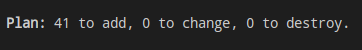
\includegraphics[width=0.67\columnwidth]{figura9.png}
              \caption{Número de recursos a crear, destruir o modificar por Terraform}
              \label{fig:figura9}
          \end{figure}
          \begin{figure}[H]
              \centering
              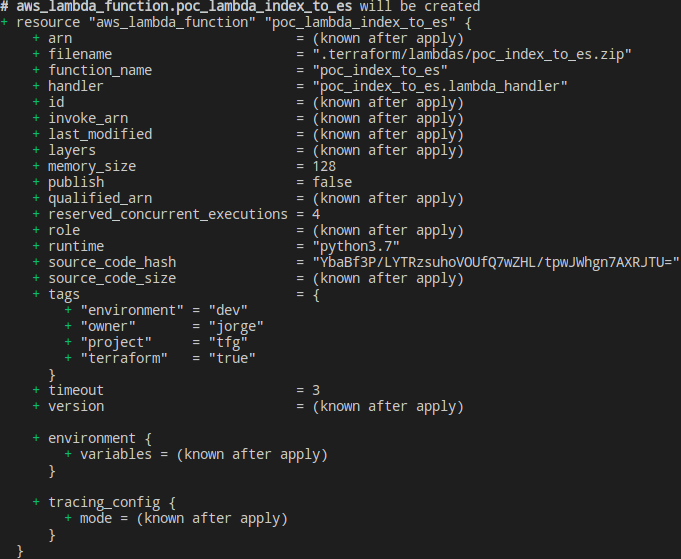
\includegraphics[width=0.67\columnwidth]{figura10.png}
              \caption{Lambda que indexa en Elasticsearch}
              \label{fig:figura10}
          \end{figure}
          \begin{figure}[H]
              \centering
              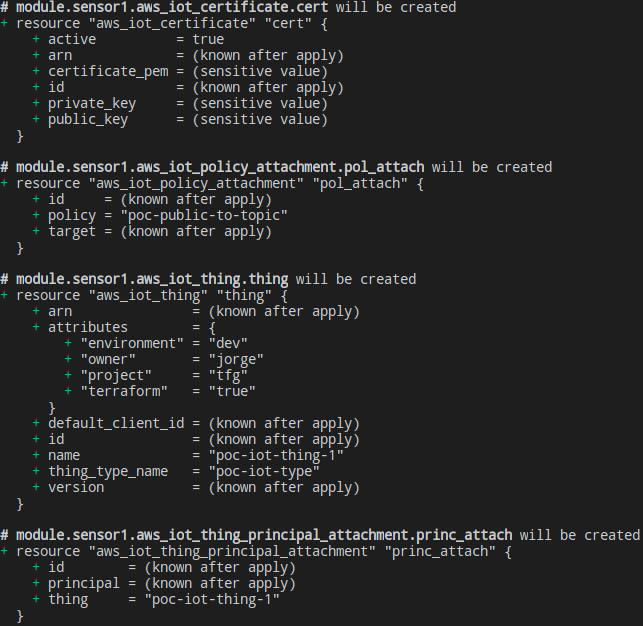
\includegraphics[width=0.67\columnwidth]{figura11.png}
              \caption{Recursos que se crearán para uno de los cuatro sensores IoT}
              \label{fig:figura11}
          \end{figure}
          \begin{figure}[H]
              \centering
              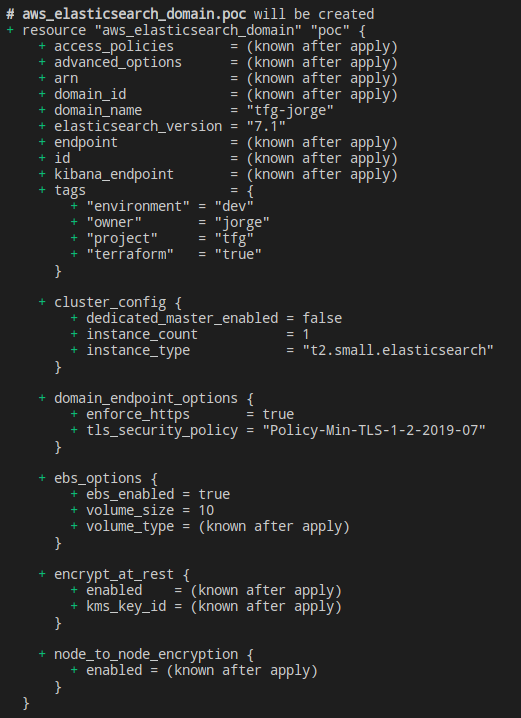
\includegraphics[width=0.67\columnwidth]{figura12.png}
              \caption{Muestra del terraform plan para el recurso Elasticsearch Service}
              \label{fig:figura12}
          \end{figure}

    \item Una vez validado y aplicado el plan de Terraform, se ejecutará el \textit{terraform apply}. La salida de Terraform una vez terminado el proceso de aplicar los cambios se muestra en la siguiente figura:
          \begin{figure}[H]
              \centering
              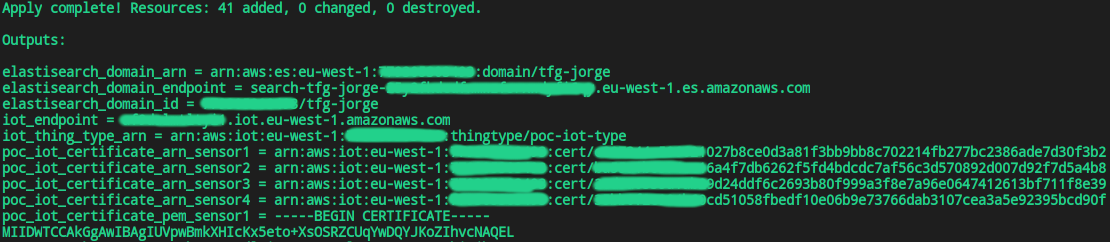
\includegraphics[width=0.7\columnwidth]{figura13.png}
              \caption{Resultado del comando terraform apply (Censurados los datos sensibles)}
              \label{fig:figura13}
          \end{figure}

    \item El siguiente paso es almacenar las variables de salida Terraform que se muestran en la figura anterior. Para ello, el script launch\_tfg.sh invoca al script save\_outputs\_terraform.py. Este script guarda los \textit{outputs} que son necesarios. Estos son (no se muestra el contenido de los archivos creados por seguridad):
          \begin{figure}[H]
              \centering
              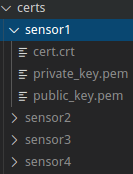
\includegraphics[width=0.3\columnwidth]{figura14.png}
              \caption{Certificados de las IoT Things desplegadas}
              \label{fig:figura14}
          \end{figure}

          \begin{figure}[H]
              \centering
              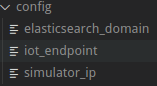
\includegraphics[width=0.3\columnwidth]{figura15.png}
              \caption{Parámetros de configuración}
              \label{fig:figura15}
          \end{figure}

    \item El último paso del despliegue es subir los archivos del simulador a la instancia que lo va a ejecutar, ejecutar el comando \textit{Docker build} y ejecutar el comando \textit{docker run}. La salida de dichos pasos puede observarse en las siguientes figuras:
          \begin{figure}[H]
              \centering
              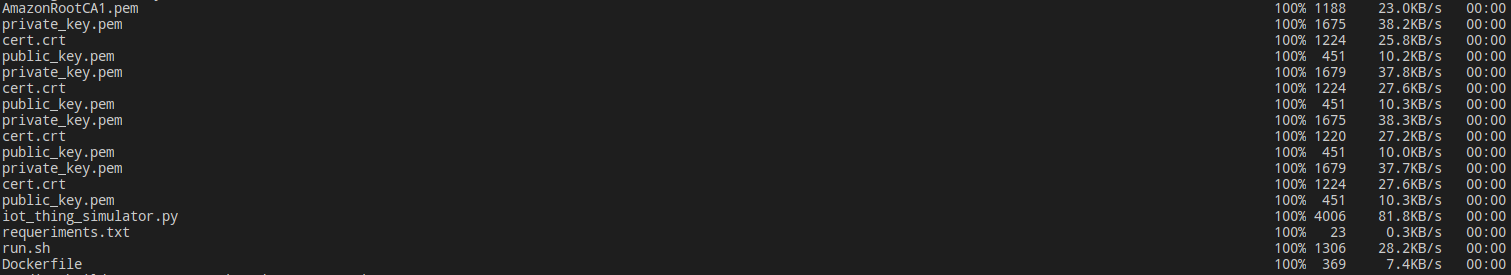
\includegraphics[width=0.7\columnwidth]{figura16.png}
              \caption{Archivos copiados mediante scp a la instancia que ejecutará el simulador}
              \label{fig:figura16}
          \end{figure}
          \begin{figure}[H]
              \centering
              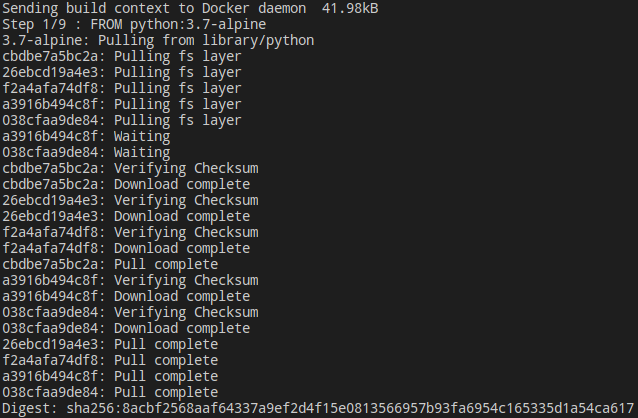
\includegraphics[width=0.7\columnwidth]{figura17.png}
              \caption{docker build 1/2}
              \label{fig:figura17}
          \end{figure}
          \begin{figure}[H]
              \centering
              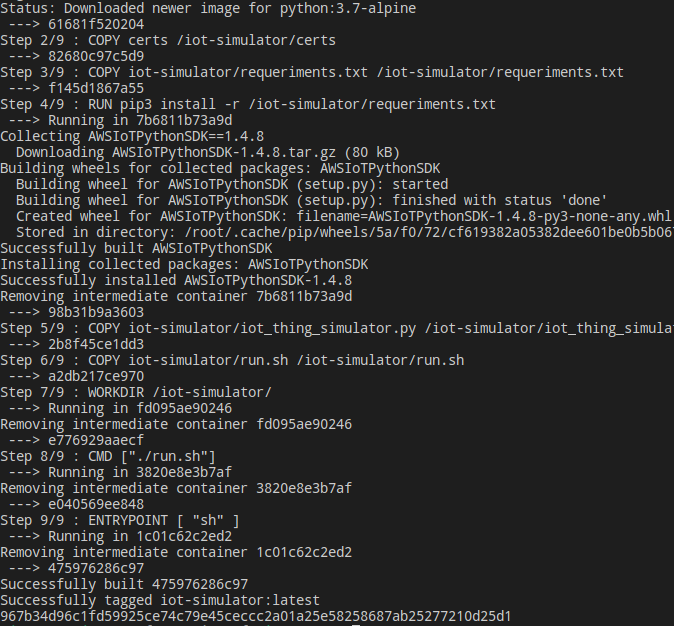
\includegraphics[width=0.7\columnwidth]{figura18.png}
              \caption{docker build 2/2 y docker run}
              \label{fig:figura18}
          \end{figure}
\end{enumerate}

\paragraph{}
Al finalizar toda esta serie de pasos, la infraestructura final estará desplegada y el simulador comenzará a enviar datos con una frecuencia entre cinco y diez segundos. En una implementación real, esta frecuencia sería mucho más baja ya que no son necesarios datos separados por tan poco tiempo en un entorno real. Se ha decidido implementar de esta forma para que sea ágil poder mostrar el funcionamiento de la solución.

\end{document}
